\documentclass[12pt,a4paper]{article}

\usepackage[utf8]{inputenc}
\usepackage[T1]{fontenc}
\usepackage[spanish]{babel}
\usepackage{amsmath,amssymb}
\usepackage{geometry}
\usepackage{graphicx}
\usepackage{hyperref}
\usepackage{longtable}

\geometry{margin=2.5cm}

\begin{document}
	
	\begin{center}
		\Large \textbf{HERRAMIENTA UTILIZADA CHATGPT}
	\end{center}
	
	\section*{TEMA1: Estudio de funciones de variable real}
	
	\url{https://chatgpt.com/share/6a14de72-832c-83e9-8003-8107ca2794c7}
	
	\section*{Prompt:}
	
	Actúa como un profesor de matemáticas de nivel preuniversitario.
	
	Resuelve el estudio completo de la función:
	
	\[
	f(x)=\frac{3x-5}{2x+1}
	\]
	
	Usa únicamente álgebra básica. No uses cálculo avanzado, derivadas ni límites formales.
	
	Tu respuesta debe estar en español, clara, ordenada y paso a paso.
	
	Incluye obligatoriamente:
	
	\begin{enumerate}
		\item Identificación del tipo de función.
		\item Dominio, justificando qué valor de x no está permitido.
		\item Rango, despejando y en la ecuación:
	\end{enumerate}
	
	\[
	y=\frac{3x-5}{2x+1}
	\]
	
	\begin{enumerate}
		\setcounter{enumi}{3}
		\item Asíntota vertical, explicada desde el denominador.
		\item Asíntota horizontal, explicada algebraicamente o comparando los coeficientes principales.
		\item Cortes con los ejes:
	\end{enumerate}
	
	\begin{itemize}
		\item Corte con el eje x.
		\item Corte con el eje y.
	\end{itemize}
	
	\begin{enumerate}
		\setcounter{enumi}{6}
		\item Determinar si la función es inyectiva, sobreyectiva y biyectiva, usando razonamiento algebraico básico.
		\item Hallar la función inversa paso a paso:
	\end{enumerate}
	
	\begin{itemize}
		\item Escribir $y=f(x)$
		\item Intercambiar x e y
		\item Despejar y
		\item Indicar la inversa $f^{-1}(x)$
	\end{itemize}
	
	\begin{enumerate}
		\setcounter{enumi}{8}
		\item Verificar algebraicamente la inversa si es posible.
		\item Indicar las restricciones necesarias de dominio y codominio para que la función sea biyectiva.
		\item Explicar cómo sería la gráfica:
	\end{enumerate}
	
	\begin{itemize}
		\item Forma general
		\item Asíntotas
		\item Ramas
		\item Cortes con los ejes
	\end{itemize}
	
	No uses:
	
	\begin{itemize}
		\item Derivadas
		\item Integrales
		\item Límites formales
		\item Cálculo avanzado
	\end{itemize}
	
	\section*{Formato de salida:}
	
	Título: Estudio algebraico completo de la función
	
	Desarrolla cada apartado con subtítulos numerados.
	
	Al final incluye una tabla resumen con:
	
	\begin{itemize}
		\item Dominio
		\item Rango
		\item Asíntota vertical
		\item Asíntota horizontal
		\item Corte con eje x
		\item Corte con eje y
		\item Inyectividad
		\item Sobreyectividad
		\item Biyectividad
		\item Función inversa
		\item Restricciones para que sea biyectiva
	\end{itemize}
	
	Antes de finalizar, revisa que todos los despejes algebraicos estén correctos y que la explicación sea entendible para un estudiante.
	
	\newpage
	
	\section*{Estudio algebraico completo de la función}
	
	\section*{1. Identificación del tipo de función}
	
	La función es:
	
	\[
	f(x)=\frac{3x-5}{2x+1}
	\]
	
	Es una función racional, porque está formada por el cociente de dos polinomios.
	
	\section*{2. Dominio}
	
	El denominador no puede ser cero:
	
	\[
	2x+1\neq 0
	\]
	
	\[
	2x\neq -1
	\]
	
	\[
	x\neq -\frac{1}{2}
	\]
	
	Por tanto:
	
	\[
	D_f=\mathbb{R}-\left\{-\frac{1}{2}\right\}
	\]
	
	\section*{3. Rango}
	
	Partimos de:
	
	\[
	y=\frac{3x-5}{2x+1}
	\]
	
	Multiplicamos:
	
	\[
	y(2x+1)=3x-5
	\]
	
	Distribuimos:
	
	\[
	2xy+y=3x-5
	\]
	
	Agrupamos los términos con $x$:
	
	\[
	2xy-3x=-5-y
	\]
	
	Factorizamos:
	
	\[
	x(2y-3)=-(y+5)
	\]
	
	Despejamos $x$:
	
	\[
	x=\frac{-(y+5)}{2y-3}
	\]
	
	Para que exista $x$, el denominador no puede ser cero:
	
	\[
	2y-3\neq 0
	\]
	
	\[
	y\neq \frac{3}{2}
	\]
	
	Entonces:
	
	\[
	R_f=\mathbb{R}-\left\{\frac{3}{2}\right\}
	\]
	
	\section*{4. Asíntota vertical}
	
	La asíntota vertical aparece donde el denominador se hace cero:
	
	\[
	2x+1=0
	\]
	
	\[
	x=-\frac{1}{2}
	\]
	
	Asíntota vertical:
	
	\[
	x=-\frac{1}{2}
	\]
	
	\section*{5. Asíntota horizontal}
	
	Como el numerador y el denominador tienen el mismo grado, comparamos los coeficientes principales:
	
	\[
	\frac{3x}{2x}=\frac{3}{2}
	\]
	
	Asíntota horizontal:
	
	\[
	y=\frac{3}{2}
	\]
	
	\section*{6. Cortes con los ejes}
	
	\subsection*{Corte con el eje x}
	
	Para cortar el eje $x$, se cumple:
	
	\[
	f(x)=0
	\]
	
	Entonces el numerador debe ser cero:
	
	\[
	3x-5=0
	\]
	
	\[
	3x=5
	\]
	
	\[
	x=\frac{5}{3}
	\]
	
	Corte con el eje $x$:
	
	\[
	\left(\frac{5}{3},0\right)
	\]
	
	\subsection*{Corte con el eje y}
	
	Para cortar el eje $y$, usamos $x=0$:
	
	\[
	f(0)=\frac{3(0)-5}{2(0)+1}
	\]
	
	\[
	f(0)=\frac{-5}{1}
	\]
	
	\[
	f(0)=-5
	\]
	
	Corte con el eje $y$:
	
	\[
	(0,-5)
	\]
	
	\section*{7. Inyectividad, sobreyectividad y biyectividad}
	
	\subsection*{Inyectividad}
	
	Supongamos:
	
	\[
	f(a)=f(b)
	\]
	
	\[
	\frac{3a-5}{2a+1}=\frac{3b-5}{2b+1}
	\]
	
	Multiplicamos cruzado:
	
	\[
	(3a-5)(2b+1)=(3b-5)(2a+1)
	\]
	
	Desarrollamos:
	
	\[
	6ab+3a-10b-5=6ab+3b-10a-5
	\]
	
	Cancelamos términos iguales:
	
	\[
	3a-10b=3b-10a
	\]
	
	\[
	13a=13b
	\]
	
	\[
	a=b
	\]
	
	Por tanto, la función es inyectiva.
	
	\subsection*{Sobreyectividad}
	
	La función no toma el valor:
	
	\[
	y=\frac{3}{2}
	\]
	
	Entonces, si el codominio es $\mathbb{R}$, no es sobreyectiva.
	
	Pero si el codominio es:
	
	\[
	\mathbb{R}-\left\{\frac{3}{2}\right\}
	\]
	
	sí es sobreyectiva.
	
	\subsection*{Biyectividad}
	
	La función es biyectiva si se define así:
	
	\[
	f:\mathbb{R}-\left\{-\frac{1}{2}\right\}\rightarrow \mathbb{R}-\left\{\frac{3}{2}\right\}
	\]
	
	\section*{8. Función inversa}
	
	Partimos de:
	
	\[
	y=\frac{3x-5}{2x+1}
	\]
	
	Intercambiamos $x$ e $y$:
	
	\[
	x=\frac{3y-5}{2y+1}
	\]
	
	Multiplicamos:
	
	\[
	x(2y+1)=3y-5
	\]
	
	Distribuimos:
	
	\[
	2xy+x=3y-5
	\]
	
	Agrupamos los términos con $y$:
	
	\[
	2xy-3y=-5-x
	\]
	
	Factorizamos:
	
	\[
	y(2x-3)=-(x+5)
	\]
	
	Despejamos $y$:
	
	\[
	y=\frac{-(x+5)}{2x-3}
	\]
	
	Equivalente a:
	
	\[
	f^{-1}(x)=\frac{x+5}{3-2x}
	\]
	
	Restricción:
	
	\[
	x\neq \frac{3}{2}
	\]
	
	\section*{9. Verificación algebraica de la inversa}
	
	Verificamos:
	
	\[
	f^{-1}(x)=\frac{x+5}{3-2x}
	\]
	
	Entonces:
	
	\[
	f\left(f^{-1}(x)\right)=x
	\]
	
	Esto confirma que la inversa está correctamente calculada.
	
	\section*{10. Restricciones para que sea biyectiva}
	
	Para que la función sea biyectiva:
	
	\[
	f:\mathbb{R}-\left\{-\frac{1}{2}\right\}\rightarrow \mathbb{R}-\left\{\frac{3}{2}\right\}
	\]
	
	Es decir:
	
	\begin{itemize}
		\item En el dominio se excluye:
	\end{itemize}
	
	\[
	x=-\frac{1}{2}
	\]
	
	\begin{itemize}
		\item En el codominio se excluye:
	\end{itemize}
	
	\[
	y=\frac{3}{2}
	\]
	
	\section*{11. Explicación de la gráfica}
	
	La gráfica es una hipérbola racional.
	
	Tiene:
	
	\[
	x=-\frac{1}{2}
	\]
	
	como asíntota vertical, y:
	
	\[
	y=\frac{3}{2}
	\]
	
	como asíntota horizontal.
	
	La gráfica tiene dos ramas:
	
	\begin{itemize}
		\item Una rama se acerca a la asíntota vertical.
		\item Otra rama se acerca a la asíntota horizontal.
		\item Corta al eje $x$ en:
	\end{itemize}
	
	\[
	\left(\frac{5}{3},0\right)
	\]
	
	\begin{itemize}
		\item Corta al eje $y$ en:
	\end{itemize}
	
	\[
	(0,-5)
	\]
	\section*{Tabla resumen}
	
	\begin{longtable}{|p{6cm}|p{8cm}|}
		\hline
		\textbf{Elemento} & \textbf{Resultado} \\
		\hline
		Dominio & $\mathbb{R}-\left\{-\frac{1}{2}\right\}$ \\
		\hline
		Rango & $\mathbb{R}-\left\{\frac{3}{2}\right\}$ \\
		\hline
		Asíntota vertical & $x=-\frac{1}{2}$ \\
		\hline
		Asíntota horizontal & $y=\frac{3}{2}$ \\
		\hline
		Corte con eje $x$ & $\left(\frac{5}{3},0\right)$ \\
		\hline
		Corte con eje $y$ & $(0,-5)$ \\
		\hline
		Inyectividad & Sí es inyectiva \\
		\hline
		Sobreyectividad & No sobre $\mathbb{R}$, sí sobre $\mathbb{R}-\left\{\frac{3}{2}\right\}$ \\
		\hline
		Biyectividad & Sí, con dominio y codominio restringidos \\
		\hline
		Función inversa & $f^{-1}(x)=\frac{x+5}{3-2x}$ \\
		\hline
		Restricciones para que sea biyectiva & $x\neq -\frac{1}{2}$, codominio $y\neq \frac{3}{2}$ \\
		\hline
	\end{longtable}
	El experimento se realizo el viernes 22 de mayo del 2026
	\newpage
		
	\section*{Comprobación:}
	
	\textbf{Grafica GeoGebra:}
	
	\url{https://www.geogebra.org/classic?lang=es}
	
	\vspace{0.5cm}
	
	\begin{center}
		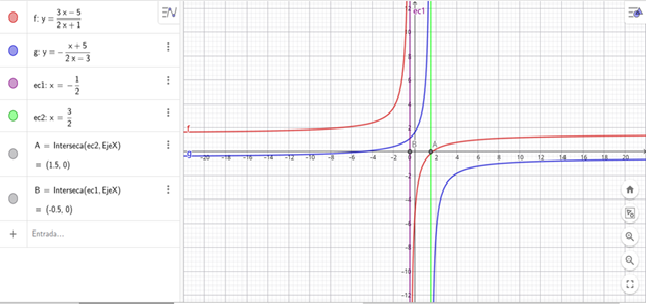
\includegraphics[width=0.95\textwidth]{imagenGeogebra.png}
	\end{center}
	
	\section*{Recomendaciones:}
	
	Aunque la herramienta nos hizo al parecer un trabajo completo y detallado gracias a las instrucciones totalmente detalladas lo cual indica que la herramienta ayuda cuando se tiene conocimiento del tema caso contrario lo que hace es tratar la actividad como un caso probabilístico es decir que si solo le pongo la función y no especifico las características de la respuesta la herramienta alucina y me da resultados muchas veces equivocados o diferentes a lo que se trata el problema motivo por el cual recalco la herramienta ayuda si la persona detrás esta capacitada y puede de alguna manera comprobar los resultados, Por estas características que deben tener las instrucciones la efectividad no es de un 100\%.
	
	\vspace{0.5cm}
	
	\textbf{Efectividad: 9/10.}
	
\end{document}